\documentclass[a4paper, 10pt]{article}
%\documentclass[a4paper,10pt]{article}

%\usepackage{frontmatter}

\bibliographystyle{alpha}

\usepackage{amsfonts}
\usepackage[left=3cm,top=2cm,right=3cm,nohead,nofoot]{geometry}
\usepackage{psfig}
\usepackage{epsfig}
\usepackage{pstricks}
\usepackage{pst-node}
%\usepackage{amsmath}
%\usepackage{amssymb}

%opening
%\title{Searching for stable states in repeated games.}
%\author{Guillaume}

\usepackage{xypic}
\usepackage{graphicx}
\usepackage{subfigure}

\pagestyle{empty}

\newcommand{\comment}[1]{\textbf{(#1)}}

% To use psmatrix like murphyk. Straight from his thesis.
\newcommand{\hidden}[1]{\pscirclebox{#1}}
\newcommand{\Dhidden}[1]{\psframebox{#1}}
\newcommand{\obs}[1]{\pscirclebox[fillstyle=solid,fillcolor=lightgray]{#1}}

\begin{document}

%\setlength{\baselineskip}{1.2\baselineskip}
\setlength{\parindent}{0pt}
\setlength{\parskip}{2ex plus 0.5ex minus 0.2ex}

%\setlength{\textwidth}{7.0in}
%\setlength{\oddsidemargin}{0.0in}
%\setlength{\evensidemargin}{0.0in}
%\headheight 1.0in
%\topmargin 0.5in
%\textheight 9.0in
%\footheight 1.0in 


%\maketitle

\begin{Large}\textbf{Causality and Noncompliance in Drug Testing}\end{Large}

by Guillaume Alain

\begin{abstract}
We present the basics for the language of causality the do-calculus, introduced
by Pearl. We show how traditional DAGs can be used to convey causality
relations and discuss the difference between experimental and artifically
generated data. We go over the analysis of compliance for drug testing from
Pearl and Chickering and discuss the problems with a posterior distribution for
a non-identifiable quantity. We provide additional graphs to get some insight
into the Gibbs sampling used.
\end{abstract}

%\Huge
%\psset{unit=4,arrowscale=2}

\section{Introduction}

\begin{quote}
\emph{I have heard tell that the people of two villages once destroyed one
another, because of a drop of honey. [...] He stopped at the shop of an oilman
and offered him the honey for sale and he bought it. Then he emptied it out of
the skin, that he might see it, and in the act a drop fell to the ground,
whereupon the flies flocked to it and a bird swooped down upon the flies. Now
the oilman had a cat, which sprang upon the bird, and the huntsman’s dog, seeing
the cat, sprang upon it and slew it; whereupon the oilman sprang upon the dog
and slew it, and the huntsman in turn sprang upon the oilman and slew him.
} \flushright{One Thousand and One Nights,
translated by Sir Richard Burton}
\end{quote}

%Causality is an ill-defined concept that plays an important role in our
%understanding of the world. A plant grows towards the sun, but the sun couldn't
%care less about the plant. Moving the plant won't affect the sun, but moving
%the light source will affect the growth of the plant. Classical statistics are
%concerned with modeling correlations, and causality is concerned with
%mechanisms involving the correlated quantities.

%The essence of causality  has to do with the possibility of performing
%interventions on the system at the time when the values of some variables.
%Classical statistics don't provide an algebraic framework to talk about
%these interventions so it's not surprise that they recommend that we be very
%careful about extracting causal relations from data. Without a proper
%mathematical language to describe interventions, we are left with the burden of
%using our common sense to determine how to interpret statistics.

%	\comment{Basically, the approach that we will use here is to define
%causality in
%a simple mathematical context and leave out the question of whether or not this
%actually translates well into reality. I am personally convinced that the same
%thing is happening with the notion of randomness. Randomness in easily defined
%in terms of measuring a space, but as soon as we start rolling real dice we
%encounter unsolvable problems about determinism in the universe. What matters
%is
%that our abstract theory, when applied to the real world, produces good
%results,
%and this is what our notion of causality will do.}

One of the most important lessons to be learned in statistics in that
correlation does not imply causality. Statistics do not make claims about
causality, and they would be rather useless if it were not
for the fact that we can sometimes supply the intuition to deduce some form of
causal relations responsible for the observed correlations. In this paper we
will look
at a language, the \textit{do-calculus}, whose purpose is to serve as a formal
tool to perform causal deductions symbolically.

As we should expect, it does not answer previously unanswerable questions and it
does not magically inject causal meaning into data. Like everything else in
mathematics, it is only a formal tool to attack larger problems by organizing
our thoughts properly and communicating them effectively.

We start in section \ref{sec:basics} by introducing the basic tools of causality
required to understand the material. We assume that the reader is relatively
confortable with graphical models used in Bayesian inference. In section
\ref{sec:drugtesting} we explain the purpose of \cite{pearl2000cmr} and
\cite{chickering1997cst} in the context of drug testing, we reproduce their
results and we provide some additional graphs that,
we think, offer an interesting way to visualize their Gibbs sampling.

\section{Basic principles of causality}
\label{sec:basics}

%	Causality is one of the topics that philosophers like to discuss. On one
%side, we are unable to define the concept properly and we might be tempted to
%reject it altogether, but on the other side, we can all admit that it's
%something fundamental in our decision-making processes.

The most natural way to construct a DAG representing a joint distribution
over some variables is to ask in what order would Nature assign their values,
and on what quantities those variables depend at the moment that they are
sampled. We can use our causal intuition to supply basic independance
assertions about the variables and then the d-separation machinery to
deduce the unintuitive relationships.

Consider the popular example involving clouds $C$, a sun-powered
sprinkler $S$, rain $R$ and potentially wet grass $W$. Before any mention of
the parameters involved in the joint distribution we can easily sketch the
little diagram in Figure \ref{fig:three_possibilities_for_sprinkler}a. Other
valid DAGs can be identified (see Figure
\ref{fig:three_possibilities_for_sprinkler}b,c) and they are just as good in
terms of modeling statistical correlations and independance relationships.

\begin{figure}[htb!]
%\centerline{
%\psset{xunit=10mm,yunit=10mm}
\begin{center}
\begin{tabular}{ccc}
\psset{arrows=->,arrowscale=2}
\psset{arcangle=45}
\begin{psmatrix}[rowsep=4mm,colsep=6mm]
			& [name=C]\hidden{$C$} 	& \\ [0pt]
[name=R]\hidden{$R$} 	& 			& [name=S]\hidden{$S$} \\
			& [name=W]\hidden{$W$} 	&
\ncline{C}{R}
\ncline{C}{S}
\ncline{R}{W}
\ncline{S}{W}
\end{psmatrix}
&
\psset{arrows=->,arrowscale=2}
\psset{arcangle=45}
\begin{psmatrix}[rowsep=4mm,colsep=6mm]
			& [name=C]\hidden{$C$} 	& \\ [0pt]
[name=R]\hidden{$R$} 	& 			& [name=S]\hidden{$S$} \\
			& [name=W]\hidden{$W$} 	&
\ncline{C}{R}
\ncline{S}{C}
\ncline{R}{W}
\ncline{S}{W}
\end{psmatrix}
&
\psset{arrows=->,arrowscale=2}
\psset{arcangle=45}
\begin{psmatrix}[rowsep=4mm,colsep=6mm]
			& [name=C]\hidden{$C$} 	& \\ [0pt]
[name=R]\hidden{$R$} 	& 			& [name=S]\hidden{$S$} \\
			& [name=W]\hidden{$W$} 	&
\ncline{R}{C}
\ncline{C}{S}
\ncline{R}{W}
\ncline{S}{W}
\end{psmatrix} \\
(a) & (b) & (c)
\end{tabular}
\end{center}
\caption{
(a) The DAG based on causal intuition. (b) \& (c) The equivalent DAGs in terms
of the conditional independance relations encoded.
 Those three DAGs are equivalent when we model statistical correlation, but
they are not equivalent when DAGs are used to model a causal mechanism allowing
 interventions.
}
\label{fig:three_possibilities_for_sprinkler}
\end{figure}

However, if we were to ask what would happen if we were to intervene by
turning off the sprinkler manually, or by pouring a tank of water on the grass,
only DAG (a) would be useful because it describes more than statistical
correlations : it describes the mechanism by which the objects really influence
each other.

Pearl points out in \cite{pearl2000cmr} that we are already attributing a
special meaning
to \ref{fig:three_possibilities_for_sprinkler} (a), often preferring it over the
alternatives (b), (c) even in the context of modeling correlation. He argues
that a new formal language is needed to describe the concept of interventions.

The basic operation featured in his \textit{do-calculus} is an intervention
on a node $X$ in a given DAG, denoted by do$(X=x)$. It corresponds
to removing
of all arrows going into $X$, treating $X=x$ as an observed variable and
performing the usual Bayesian inference on the resulting graph. We can perform
interventions on any number of nodes in addition to having observed or hidden
nodes as usual.

Interventions are defined in terms of a particular DAG to which we will
refer here as the ``causal graph''. We select a causal
graph that represents sufficiently well, in our judgement, the process by
which Nature generates the samples. If such a graph can be found, the
\textit{do-calculus} interventions will match the potential real-life
interventions. This provides us a powerful symbolic
machinery to model the unintuitive consequences of real-life interventions.

Returning to the example of the wet grass, we compare in figure
\ref{fig:interventions_on_sprinkler} the causal model, the effects
of $do(S=s)$, the effects of $do(W=w)$ and the usual conditional distribution
with $W=w$.
The formulas for the pdfs are the following :

\begin{tabular}{crcl}
(a) & $p(C,R,S,W)$ & = & $p(C)\ p(R|C)\ p(S|C)\ p(W|R,S)$ \\
(b) & $p(C,R,W | do(S=s))$ & = & $p(C)\
p(R|C)\ p(W|R,S=s)$ \\
(c) & $p(C,R,S | do(W=w))$ & = & $p(C)\ p(R|C)\ p(S|C)$ \\
(d) & $p(C,R,S | W=w)$ & $\propto$ & $p(C)\ p(R|C)\ p(S|C)\ p(W=w|R,S)$
\end{tabular}

\begin{figure}[htb!]
%\centerline{
%\psset{xunit=10mm,yunit=10mm}
\begin{center}
\begin{tabular}{cccc}
\psset{arrows=->,arrowscale=2}
\psset{arcangle=45}
\begin{psmatrix}[rowsep=4mm,colsep=6mm]
			& [name=C]\hidden{$C$} 	& \\ [0pt]
[name=R]\hidden{$R$} 	& 			& [name=S]\hidden{$S$} \\ [0pt]
			& [name=W]\hidden{$W$} 	&
\ncline{C}{R}
\ncline{C}{S}
\ncline{R}{W}
\ncline{S}{W}
\end{psmatrix}
&
\psset{arrows=->,arrowscale=2}
\psset{arcangle=45}
\begin{psmatrix}[rowsep=4mm,colsep=6mm]
			& [name=C]\hidden{$C$} 	& \\ [0pt]
[name=R]\hidden{$R$} 	& 			& [name=S]\obs{$S$} \\
[0pt]
			& [name=W]\hidden{$W$} 	&
\ncline{C}{R}
\ncline{R}{W}
\ncline{S}{W}
\end{psmatrix}
&
\psset{arrows=->,arrowscale=2}
\psset{arcangle=45}
\begin{psmatrix}[rowsep=4mm,colsep=6mm]
			& [name=C]\hidden{$C$} 	& \\ [0pt]
[name=R]\hidden{$R$} 	& 			& [name=S]\hidden{$S$} \\ [0pt]
			& [name=W]\obs{$W$} 	&
\ncline{C}{R}
\ncline{C}{S}
\end{psmatrix} &
\psset{arrows=->,arrowscale=2}
\psset{arcangle=45}
\begin{psmatrix}[rowsep=4mm,colsep=6mm]
			& [name=C]\hidden{$C$} 	& \\ [0pt]
[name=R]\hidden{$R$} 	& 			& [name=S]\hidden{$S$} \\ [0pt]
			& [name=W]\obs{$W$} 	&
\ncline{C}{R}
\ncline{C}{S}
\ncline{R}{W}
\ncline{S}{W}
\end{psmatrix}\\
(a) & (b) & (c) & (d)
\end{tabular}
\end{center}
\caption{
(a) The original causal model. (b) After performing the intervention $do(S=s)$.
(c) After performing the intervention $do(W=w)$. (d) Comparing with simple
conditioning on $W=w$.
}
\label{fig:interventions_on_sprinkler}
\end{figure}

%Choosing the appropriate causal graph can be very hard. In fact, modeling
%interventions on $n$ variables might require a causal graph with a number of
%nodes of an order of magnitude above $n$. This is very problematic when

The delicate issue is whether or not we can find such a graph in which
\textit{do-calculus} interventions correspond to real-life interventions. In
some artificial settings, the correspondance can be perfect, but in most
experimental settings, the best that we can hope for are causal graphs that are
useful.

Consider the typical Bayesian models where we define a joint distribution by
means of a DAG $\mathcal{G}$ and we decide to sample from the joint in the
usual order specified by the arrows $\mathcal{G}$. We can define interventions
as little clamps put on particular nodes that refrain the sampling algorithm
from changing the value of those nodes to anything else than specified values.
In that case, the interventions can be modeled perfectly by \textit{do-calculus}
by using $\mathcal{G}$ as the causal graph.

%The reader might at this point feel that circular definitions are involved, but
%this is because \textit{do-calculus} revolves around the possibility of
%establishing a correspondance between its interventions in the abstract context
%of a causal DAG, and the real interventions found in another setting
%(experimental or artificial). The most trivial case in which the interventions
%of \textit{do-calculus} correspond to those of another setting in when that
%other setting is the above scenario with clamps on certain nodes.

%\comment{L\`a on retombe dans ce que j'ai \'ecrit dans ma premi\`ere version.}

% 	Directed acyclic graphs (DAGs) offer a way to represent in a very
% compact manner independance relationships between variables \comment{aucune
%idee
% si je dois en parler precisement}. They also provide a natural way to evaluate
% the probability of given outcomes by simply multiplying out the values for the
% conditional pdfs at those points \comment{mal dit}. They usually provide a
% simple way to sample from the joint distribution, but this is due to the fact
% that the DAGs are constructed by defining local conditional distributions that
% are relatively simple.
% 
% 	The intuitive way to create DAGs that models a joint distribution on a
% set of variables is to think about the relation between the variables in terms
% of causality (in the common sense of the word), order the variables according
%to
% their order in the chain of influence and then pick local conditional
% distributions by thinking only about the preceeding variables, assuming that
% this will be sufficient.
% 
% 	The notion of causality relies on the fact that the variables are
% generated by Nature (or us) in a particular order and that, if we were to
% intervene at some point, we could affect what is coming after that
%intervention
% with no effect on what precedes it. The whole mechanism by which the variables
% are generated is exactly what our intuition captures when we are writing down
% the DAG for the wet grass model.

\subsection{Identifiability}

	When we have access to a causal graph that can answer queries about
interventions, we can compute quantities of the form $p(A|B,do(C))$ by
performing the intervention operations described previously. We cut the arrows
going into $C$ and then we perform the usual Bayesian graphs inference to
evaluate $p(A|B,C)$ in the resulting graph.

When such a quantity involving \textit{do-calculus} can be translated into an
expression involving only classical probabilities, the quantity is said
to be \textit{identifiable}.

When we have access to a causal graph that models interventions perfectly, all
quantities are identifiable. However, there are situations in which no such
causal graph exists, even in a artificial setting. A simple example can be
constructed from the wet grass
scenario. Suppose that we were only interested in the variables $R,S$ and knew
nothing about the existence of $C,W$. In the traditional correlational DAG
setting, we can write down the joint distribution of $R,S$ as either $R
\rightarrow S$ or $R \leftarrow S$. Note
that, by using the correct causal model involving the four variables, we have
that $p(S|do(R)) = p(S)$ and $p(R|do(S)) = p(R)$. We should get that from any
valid causal model with two variables as well, if one exists.

Assuming (to reach a contradiction) that there exists a causal model with only
the nodes $S,R$, it has to be either $R \rightarrow S$ or $R \leftarrow S$. If
it was $R \rightarrow S$, we would
get that $p(S|do(R))=p(S|R)$. However, we know that $p(S|R) \neq p(S)$ so this
causal model with two variables is wrong. Having $S \rightarrow R$ leads to a
similar contradiction. The problem is that, although a DAG with $R,S$ is a
proper tool to model the correlations between $R,S$, it is insuffisant to
capture the richness of the interactions of $R,S$ in the original context where
we allow interventions.

There are situations where we have knowledge about limited parts of the actual
causal graph that Nature uses to generate the data and we can still evaluate
quantities involving \textit{do} interventions. In \cite{pearl2000cmr}, special
dotted arrows
are used to refer to the existence of hidden variables that are common
ancestors to some of the nodes of interest. Rules are introduced to evaluate
when quantities are \textit{identifiable} despite the presence of hidden
variables not explicitly represented in the causal graph.

The drug testing scenarios presented in \cite{chickering1997cst} and
\cite{pearl2000cmr} deal with a situation
in which the quantity of interest named $ACE(X\rightarrow Y)$ is not
identifiable, but where we can nevertheless establish bounds for that quantity
using linear optimization. It is also possible in that situation to use Gibbs
sampling to obtain a posterior distribution of $ACE(X\rightarrow Y)$, but as we
are dealing with a quantity not identifiable, we have to be careful in
interpreting the results.

%Consider two honest rational logicials who are bitter rivals. If they agree on
%a causal model and they collect sufficiently many samples, they should never
%disagree on conclusions concerning identifiable quantities, but they would not
%be able to agree on a value for the quantities that are not identifiable
%(unidentifiable).

\section{Modeling compliance in drug testing}
\label{sec:drugtesting}

\subsection{The setting}

	In \cite{pearl2000cmr} and \cite{chickering1997cst} is presented an
experimental drug testing setting
in which the experimenters can supply a certain drug to patients but cannot
force them to take it. The patient does have to report if he took it or not, and
at the end of the experiment his health condition is evaluated. The three
variables are labeled by $Z,X,Y$, corresponding to

\begin{tabular}{c}
the patient is given the drug ($Z=1$) or not ($Z=0$), \\
the patient is takes the drug ($X=1$) or not ($X=0$), \\
the patient is heals the drug ($Y=1$) or not ($Y=0$).
\end{tabular}

The experimenter has to rely on his good judgement to select reasonable
threshold values to represent the final condition of the patient as 0 or 1, and
to determine how much of the treatment should have been undergone by the patient
before it qualifies as 1. The premiss of this model is that there
will be a strong connection between the decision of the patients to take the
drug or not and their potential recovery.

Comparing $p(Y=1|X=1)$ and $p(Y=1|X=0)$ is not a good measure of effi
ciency for the treatment. As Chickering and Pearl explain it so well
in \cite{chickering1997cst} :

\begin{quote}
The major source of difficulty in managing and analyzing such
experiments has
been the subject noncompliance. For example, a subject in the treatment group
may experience negative side effects and will stop taking the drug.
Alternatively, if the experiment is testing a drug for a terminal disease, a
subject suspecting that he is in the control group may obtain the drug from
other sources. Imperfect compliance poses a problem because simply comparing
the fractions as above may provide a misleading estimate for how effective the
drug would be if applied uniformly to the population. For example, if those
subjects who refused to take the drug are precisely those who would have
responded adversely, the experiment might conclude that the drug is more
effective than it actually is. 
\end{quote}

\begin{figure}[htb!]
\begin{tabular}{ccc}
\psset{arrows=->,arrowscale=2}
\psset{arcangle=45}
\begin{psmatrix}[rowsep=4mm,colsep=6mm]
[name=Z]\hidden{$Z$} &		& [name=U]\psframebox[framearc=0.5]{$U=(R_X,
R_Y)$} \\ [0pt]
 	& [name=X]\hidden{$X$}	& \\ [0pt]
			& 	& [name=Y]\hidden{$Y$}
\ncline{Z}{X}
\ncline{X}{Y}
\ncline{U}{X}
\ncline{U}{Y}
\end{psmatrix} & \hspace{2cm} &
\psset{arrows=->,arrowscale=2}
\psset{arcangle=45}
\begin{psmatrix}[rowsep=4mm,colsep=6mm]
[name=Z]\hidden{$Z$} &		& [name=RY]\hidden{$R_Y$} \\ [0pt]
 	& [name=X]\obs{$X$}	& \\ [0pt]
			& 	& [name=Y]\hidden{$Y$}
\ncline{X}{Y}
\ncline{RY}{Y}
\end{psmatrix} \\
(a) & & (b)
\end{tabular}
\caption{
(a) The causal model with the unknown hidden variables $U$ expressed as a joint
$(R_X,R_Y)$. (b) The causal model after performing \textit{do}$(X)$.}
\label{fig:basic_causal_model}
\end{figure}

% \begin{figure}[htp!]
% \xymatrix{
% *+<1.5pc>[o][F-]{Z} \ar[dr] 	& 				&
% *+<1.5pc>[o][F-]{U} \ar[dl] \ar[dd]\\
% 				& *+<1.5pc>[o][F-]{X} \ar[dr]	& \\
% 				&				&
% *+<1.5pc>[o][F-]{Y}
% }
% \label{fig:basic_causal_model}
% \end{figure}

The causal model used is shown in figure \ref{fig:basic_causal_model}. Its par
ameters are chosen to be such that, given the state of the latent variables
$U$, there is a deterministic mapping from $Z$ to $X$ and from $X$ to $Y$. The
randomness comes from the fact that the latent variables are unobserved. There
are only 16 possible pairs of
mappings so the complete space of possible latent
variables $U$ can be expressed as a joint distribution
$(R_X, R_Y)
\in \{0,1,2,3\}^2$ where $R_X$ and $R_Y$ are used to classify the patients in
four possible categories each.

\begin{tabular}{rcl}
	$R_X=0$ & : &  the patient never takes the drug $(X=0)$ \\
	$R_X=1$ & : &  the patient takes the drug iff given $(X=Z)$ \\
	$R_X=2$ & : &  the patient does the opposite of what is asked
$(X=1-Z)$
\\
	$R_X=3$ & : &  the patient always takes the drug $(X=1)$ \\
	$R_Y=0$ & : &  the patient never recovers $(Y=0)$\\
	$R_Y=1$ & : &  the patient recovers iff he takes the drug $(Y=X)$\\
	$R_Y=2$ & : &  the patient recovers iff he does not take the drug
$(Y=1-X)$\\
	$R_Y=3$ & : &  the patient always recovers $(Y=1)$
\end{tabular}


We are assuming here that the patients can find access to the treatment on
their own, whether it's because they are willing to get the drug elsewhere
or because there is some sort of flexibility in the experiment. In any
case, the choice not to rule out these possibilities is a penalty on our
predictive power and not a limiting hypothesis that narrows the applications of
the model. The object of the study is to find the ``average causal effect of
$X$ on $Y$'', written as $ACE(X\rightarrow Y)$. This quantity is defined to be
\begin{eqnarray*}
ACE(X\rightarrow Y) & = & p(Y=1|do(X=1)) - p(Y=1|do(X=0)) \\
		    & = & \left[p(R_Y=1) + p(R_Y=3)\right] - \left[p(R_Y=2) +
p(R_Y=3)\right] \\
		    & = & p(R_Y=1) - p(R_Y=2)
\end{eqnarray*}
The goal is to find $ACE(X\rightarrow Y)$ using experimental data $D$ in the
form of samples $\{(Z_i, X_i, Y_i)\}_{i=1}^n$. This is where
\cite{pearl2000cmr} and
\cite{chickering1997cst} split. The first uses
the samples to estimate $p(X,Y|Z)$ and then, defining constraints on $(R_X,
R_Y)$ based on those MLE estimates, solves two linear optimization problems to
obtain an upper and lower bound on $ACE(X\rightarrow Y)$.

The second, however, points out that estimating $p(X,Y|Z)$ from small samples
might not be a good idea. Indeed, the approach detailed in \cite{pearl2000cmr}
has no way of signaling how uncertain are the bounds given because it uses
the data only to find an MLE. It does not give a posterior distribution and
would have no good prior if we had one. In \cite{chickering1997cst},
Chickering and Pearl explain how
Gibbs sampling can be used to sample effectively on the conditional distribution
of $R_X,R_Y$ given the data collected in the experiment. From those samples of
$R_X,R_Y$ we can not only estimate $ACE(X\rightarrow Y)$, but we can get a
posterior distribution.

We will omit the details of the linear optimization approach and refer the
reader to \cite{pearl2000cmr}. The Gibbs sampling method is covered in the
next section.

%We will look at both approaches in more details in the next sections, spending
%more time on the Gibbs sampling method and discussing the posterior
%distribution of $p(R_X=2) - p(R_X=1)$ obtained.

\subsection{Gibbs sampling for posterior $ACE(X\rightarrow Y)$}

Here we go over some of the examples from \cite{pearl2000cmr} and
\cite{chickering1997cst} to reproduce their
results. They use two real datasets from the medical literature and one
artificially generated dataset that has the special property of having only one
possible value for the
$ACE(X\rightarrow Y)$. Their datasets are summarized in tables with the
frequency counts for the possible values of $X,Y|Z$.

To recover datasets we sample a number $n$ of triplets of the
same relative frequency. This only garantees that we will be asymptotically
close to those frequencies. We enumerate the possible discrete states that can
be taken by $U$ as $\{1,2,\ldots, 16\}$ and we assume that all $U_i$ are drawn
from a multinomial distribution with parameter $q\in
\mathbb{R}^{16}$.

We treat that parameter $q$ as a random variable $Q$ and we put a Dirichlet
prior of hyperparameter $\alpha=(\alpha_1,\ldots, \alpha_{16})$ on it.
We get the causal graph in figure \ref{fig:causalgraphwithplates}. The only
interventions that we will study are on $Z$ and $X$ and they should match
real-life interventions sufficiently well.

\begin{figure}[htb!]
\begin{center}
\psset{arrows=->,arrowscale=2}
\psset{arcangle=45}
\begin{psmatrix}[rowsep=4mm,colsep=6mm]
[name=Zi]\obs{$Z_i$} &		& [name=Ui]\hidden{$U_i$} & [name=Q]\hidden{$Q$}
& [name=ACE]\psframebox[framearc=0.5]{$ACE(X\rightarrow Y)$} \\ [0pt]
 	& [name=Xi]\obs{$X_i$}	& & [name=alpha]\obs{$\alpha$} & \\
[0pt]
			& 	& [name=Yi]\obs{$Y_i$} & &
\ncline{Zi}{Xi}
\ncline{Xi}{Yi}
\ncline{Ui}{Xi}
\ncline{Ui}{Yi}
\ncline{Q}{Ui}
\ncline{alpha}{Q}
\ncline{Q}{ACE}
\end{psmatrix}
\end{center}
\caption{The causal model that generates the data $D=\{(Z_i, X_i,
Y_i)\}_{i=1}^n$, denoted with a plate notation. The value $ACE(X\rightarrow Y)$
can be computed deterministically with a value $Q=q$, but we will only have
access to a posterior distribution on $Q$.}
\label{fig:causalgraphwithplates}
\end{figure}





% \begin{figure}[htp!]
% \xymatrix{
%  				&				&		
% 			& *+<1.5pc>[o][F-]{Q} \ar[dl] \ar[drrr]	& {\bullet
% \alpha} \ar[l]	&				& \\
% *+<1.5pc>[o][F-]{Z_1} \ar[dr] 	& 				&
% *+<1.5pc>[o][F-]{U_{1}} \ar[dl] \ar[dd] 	& 			
% & *+<1.5pc>[o][F-]{Z_n} \ar[dr] 	& 				&
% *+<1.5pc>[o][F-]{U_{n}} \ar[dl] \ar[dd]  \\
% 				& *+<1.5pc>[o][F-]{X_1} \ar[dr]	& 		
% 			& \ldots  			& 			
% 	& *+<1.5pc>[o][F-]{X_n} \ar[dr]	&	\\
% 				&				&
% *+<1.5pc>[o][F-]{Y_1}				&			
% &					&				&
% *+<1.5pc>[o][F-]{Y_n}
% }
% \caption{The causal model used. Note that when $U_i = u_i$ is known for a
% particular $i$, there is a deterministic relation between $Z_i, X_i, Y_i$.}
% \label{fig:causal_drug_model}
% \end{figure}

We are interested in approximating $p(Q|D)$ where $D=\{(Z_i, X_i,
Y_i)\}_{i=1}^n$. This is done using Gibbs sampling on $p(Q, U_1, \ldots,
U_n|D)$, keeping a record on the values of $Q$ sampled. We alternate between
sampling from the two following distributions :
\begin{eqnarray*}
	p(U_1, \ldots, U_n|D,Q=q) & = & \prod_{i=1}^n p(U_i|Z_i,X_i,Y_i,Q=q) \\
	p(Q|U_1=u_1, \ldots, U_n=u_n, D) & = & \textrm{Dirichlet}(\alpha_1 +
N_1,
\ldots, \alpha_{16} + N_{16})
\end{eqnarray*}
where $N_t$ is the number of patients whose observed variables $(Z_i, X_i,
Y_i)$ are compatible with the patient type $U_i=t$. For example, if $N_7$ is the
number of patients who are defiers $(R_X=2)$ and
would heal iff given the medication $(R_Y=1)$, then $N_7$ is equal to the
number of instances of $(1,0,0)$ or $(0,1,1)$ in $D$.

There is an arbitrary
decision to be made concerning the order in which the 16 states of $U=(R_X,
R_Y)$ are enumerated, but as long as we are consistent in our implementation
and we compute $ACE(X\rightarrow Y)$ from the values of $Q$ properly, we can
omit the details of the implementation.

\subsection{Practical results}

We consider here two of Pearl's example cases given in \cite{pearl2000cmr}. The
first case is an artificial setting
in which the relative frequencies are chosen to imply that
\mbox{$ACE(X\rightarrow
Y)=0.55$}. Results for different sample sizes are found in figures
\ref{fig:n=100_case0.55}, \ref{fig:n=1000_case0.55} and
\ref{fig:n=10000_case0.55}. When we produce a sample of experimental data to be
used for Gibbs
sampling, we get relative frequencies that differ a bit and, as shown in
figures \ref{fig:n=100_case0.55}c, \ref{fig:n=1000_case0.55}c, the sampled
values for the posterior $ACE(X\rightarrow Y)$ are around $0.55$. When we get
enough data, we see in figure \ref{fig:n=10000_case0.55}c that the posterior
$ACE(X\rightarrow Y)$ is very close to $0.55$.

We decided to have a look at the states of the hidden variables $U_i$
attributed to the patients during Gibbs sampling. This allows us to get a better
intuition
about the meaning of the experimental data. In figures
\ref{fig:n=1000_case0.55}b, \ref{fig:n=10000_case0.55}b we can start to see how
the only possible conclusion from the data is that no one is hurt by the
treatment. We can also see that there is a large portion of the people who
healed and would not have if it had not been for the treatment. The rest are
people whose recovery was not affected by the treatment. The part (a) of
figures \ref{fig:n=100_case0.55}, \ref{fig:n=1000_case0.55},
\ref{fig:n=10000_case0.55} are hard to interpret and were included just for
curiosity's sake.

\begin{figure}
\begin{tabular}{ccc}
 \includegraphics[width=4.5cm,height=4cm,bb=103 240 500
555]{takingtype_case0.55_n=100.eps} &
 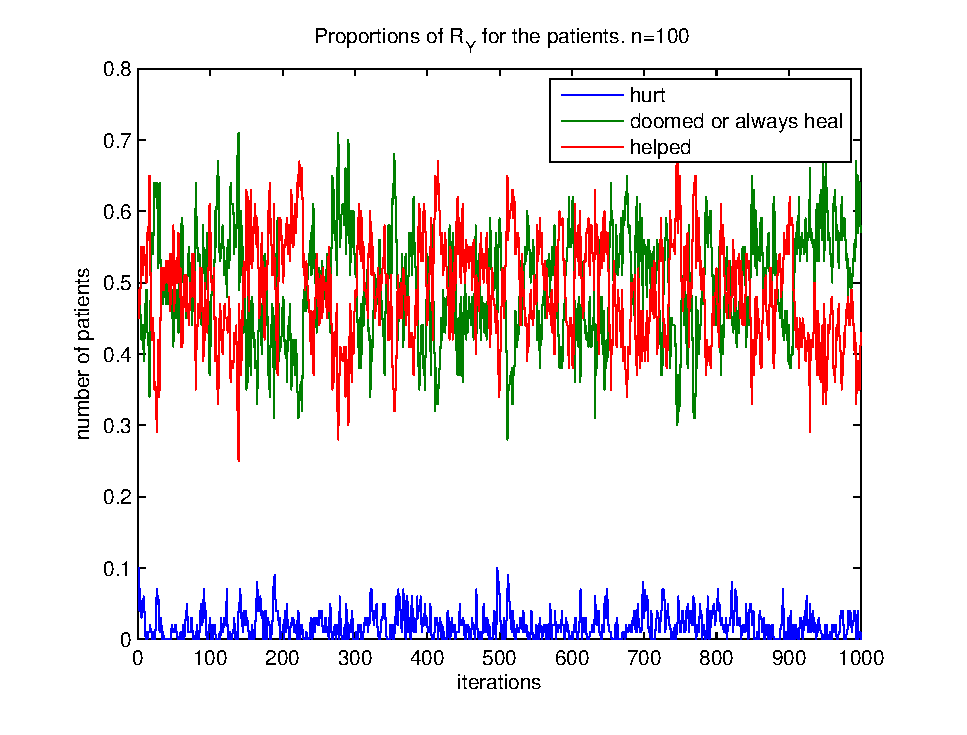
\includegraphics[width=4.5cm,height=4cm,bb=103 240 500 555]
{healingtype_case0.55_n=100.eps} &
 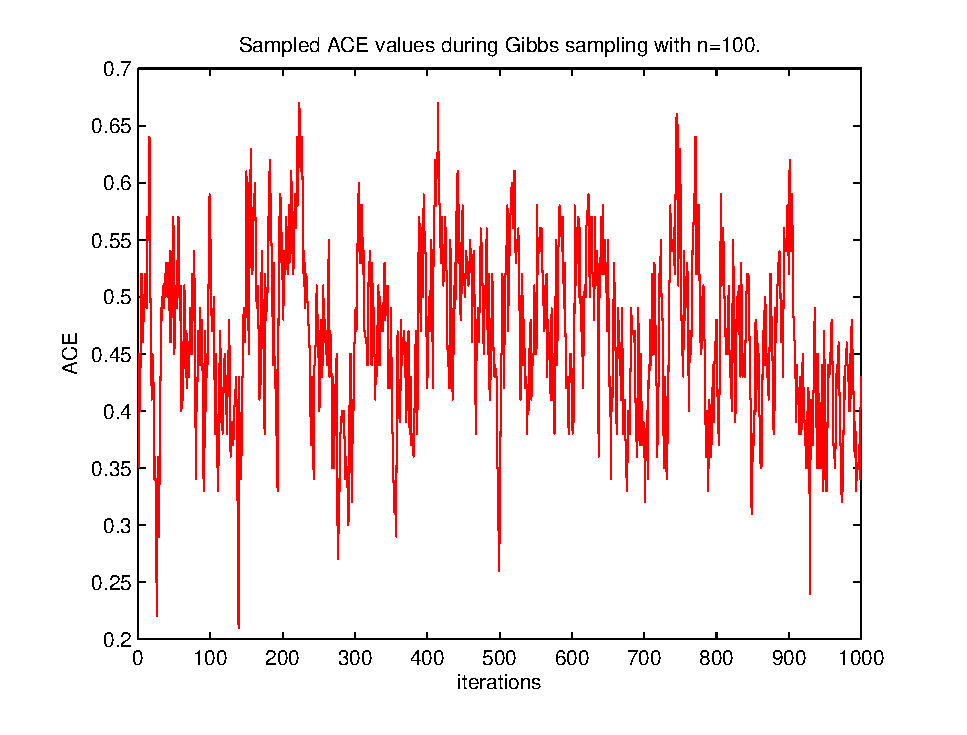
\includegraphics[width=4.5cm,height=4cm,bb=103 240
500 555]{sampledACEs_case0.55_n=100.eps} \\
(a) & (b) & (c)
\end{tabular}
\caption{Different categories of patients assigned during Gibbs sampling. We
have sampled $n=100$ patients from a distribution that should produce an
identifiable ACE of $0.55$ .}
\label{fig:n=100_case0.55}
\end{figure}

\begin{figure}
\begin{tabular}{ccc}
 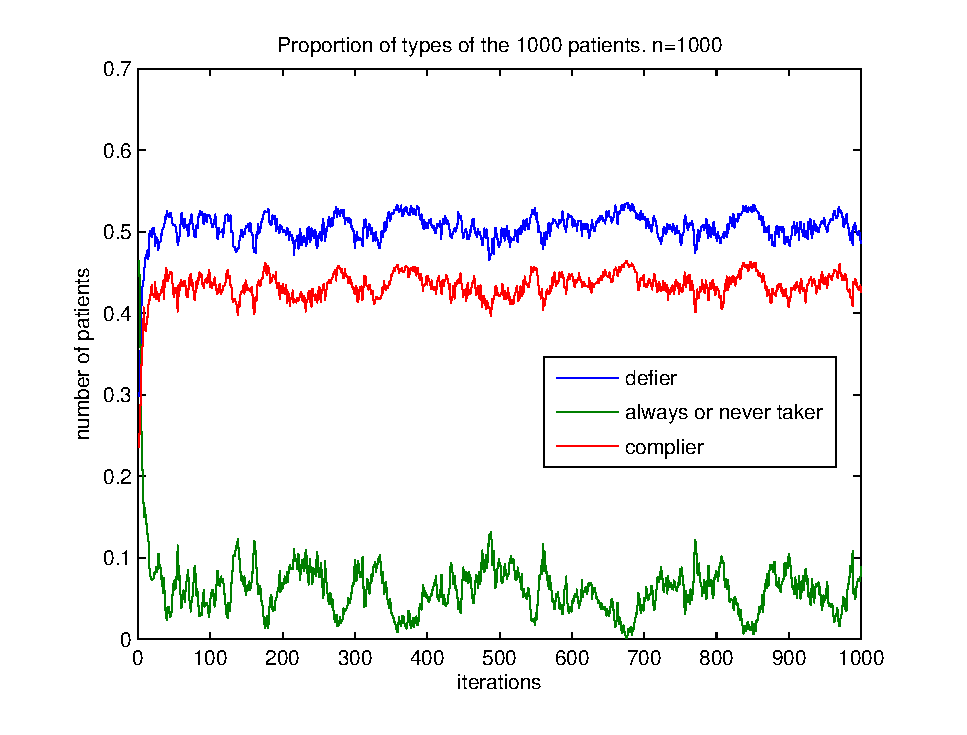
\includegraphics[width=4.5cm,height=4cm,bb=103 240 500
555]{takingtype_case0.55_n=1000.eps} &
 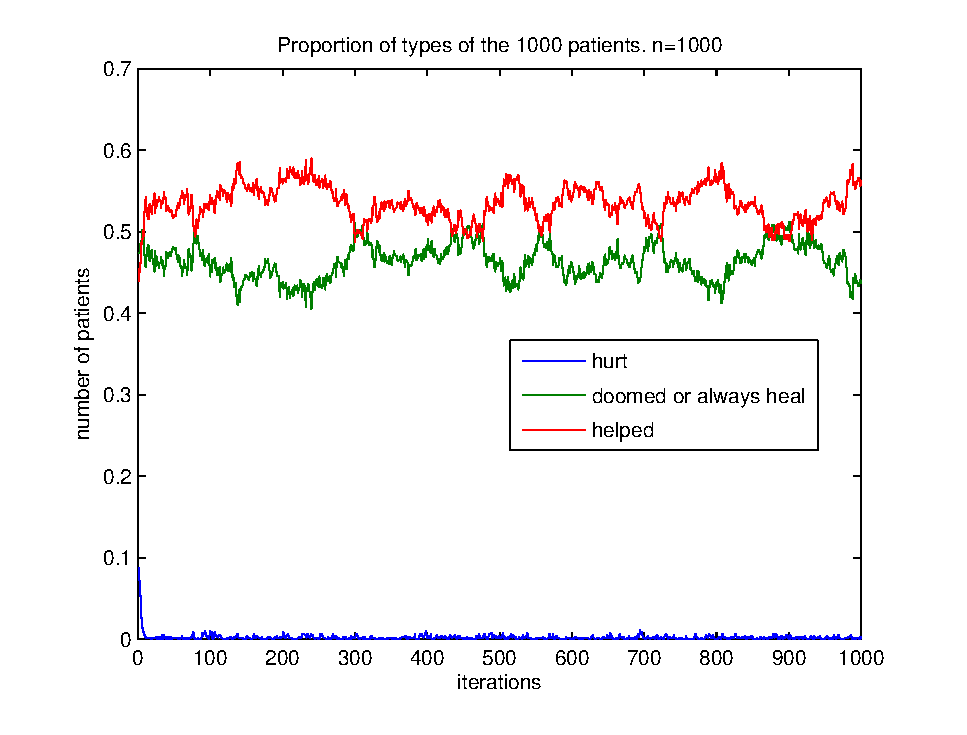
\includegraphics[width=4.5cm,height=4cm,bb=103 240 500 555]
{healingtype_case0.55_n=1000.eps} &
 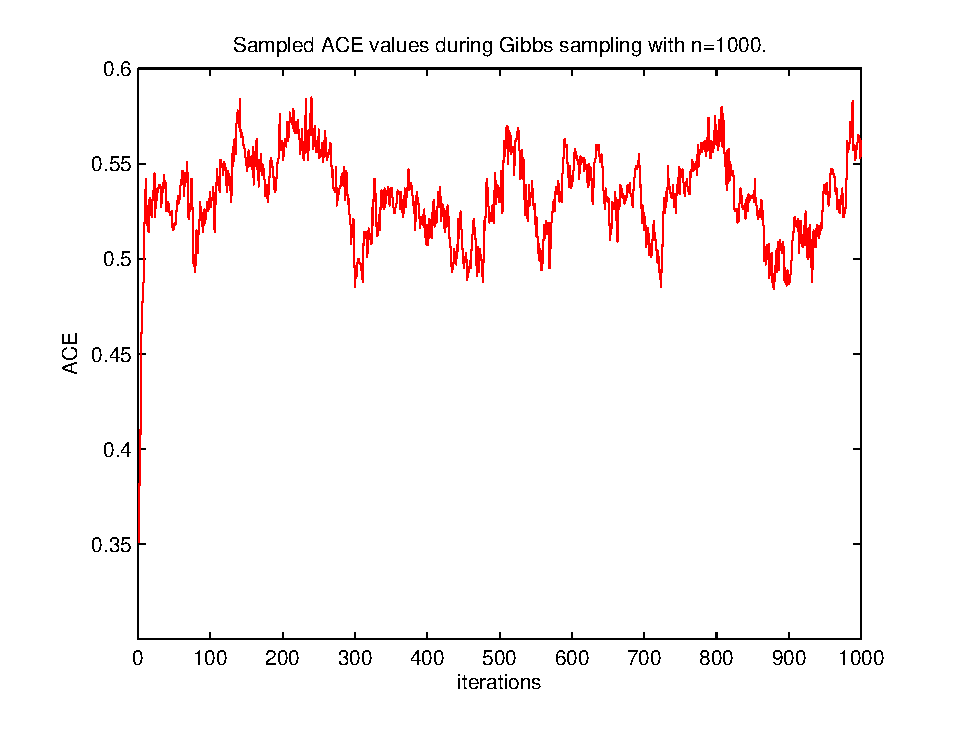
\includegraphics[width=4.5cm,height=4cm,bb=103 240
500 555]{sampledACEs_case0.55_n=1000.eps} \\
(a) & (b) & (c)
\end{tabular}
\caption{Different categories of patients assigned during Gibbs sampling. We
have sampled $n=1\ 000$ patients from a distribution that should produce an
identifiable ACE of $0.55$ .}
\label{fig:n=1000_case0.55}
\end{figure}

\begin{figure}
\begin{tabular}{ccc}
 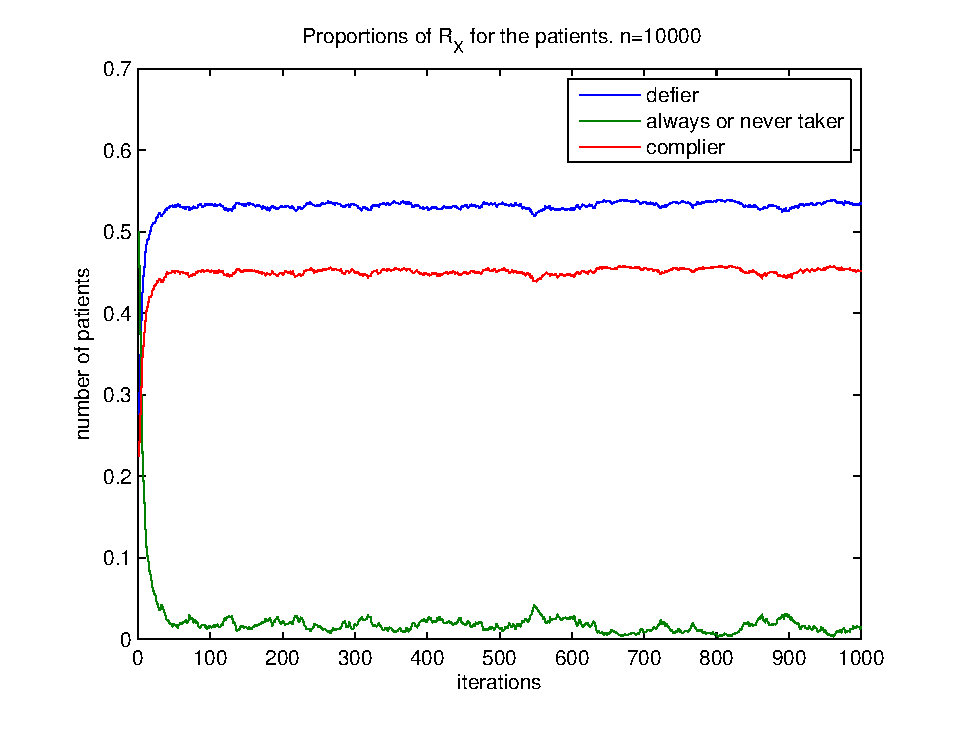
\includegraphics[width=4.5cm,height=4cm,bb=103 240 500
555]{takingtype_case0.55_n=10000.eps} &
 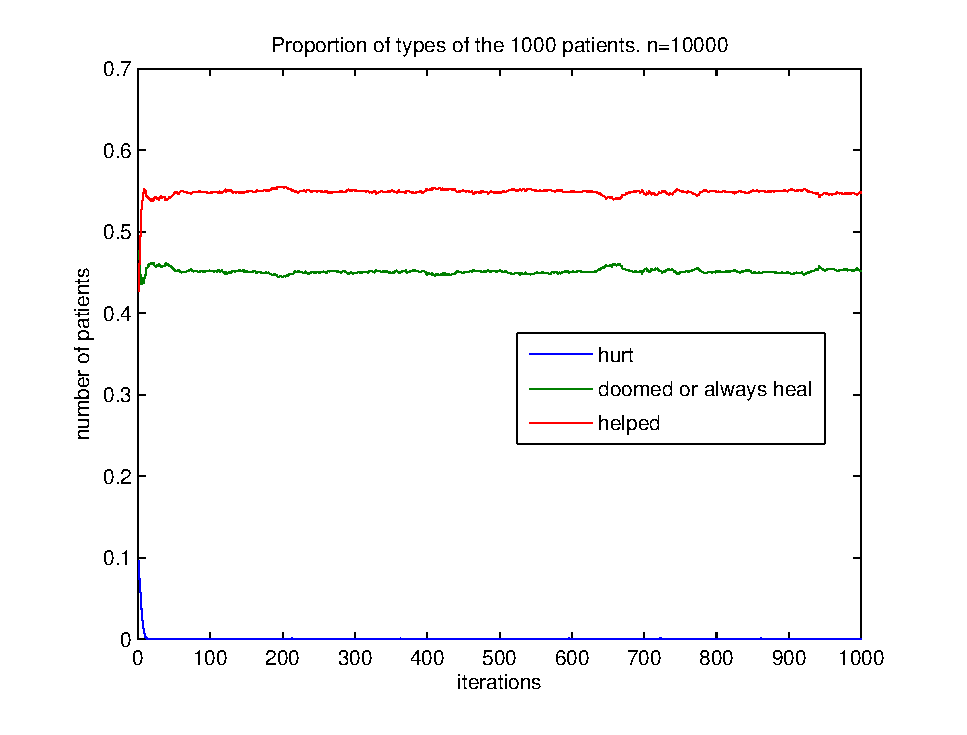
\includegraphics[width=4.5cm,height=4cm,bb=103 240 500 555]
{healingtype_case0.55_n=10000.eps} &
 \includegraphics[width=4.5cm,height=4cm,bb=103 240
500 555]{sampledACEs_case0.55_n=10000.eps} \\
(a) & (b) & (c)
\end{tabular}
\caption{Different categories of patients assigned during Gibbs sampling. We
have sampled $n=10\ 000$ patients from a distribution that should produce an
identifiable ACE of $0.55$ .}
\label{fig:n=10000_case0.55}
\end{figure}

The next case is one where it can be established with linear optimization (see
\cite{pearl2000cmr}) that $ACE(X\rightarrow Y) \in [0.38, 0.78]$. Results for
different sample sizes are found in figures
\ref{fig:n=100_case0.38_0.78}, \ref{fig:n=1000_case0.38_0.78} and
\ref{fig:n=10000_case0.38_0.78}. Again we used
experimental samples generated from a frequency table. We have to be careful
when interpreting the values sampled from the posterior $ACE(X\rightarrow Y)$.
The ``true'' $ACE(X\rightarrow Y)$ is computed from the hidden value of $Q$, but
for one set of experimental data, there are often infinitely many possible
values of $Q$ that could have generated the data. There are 15 free
parameters defining $Q$ and only 6 parameters are required to describe the
distribution $X,Y|Z$ (we usually assume that we have the same number of
$Z=0,1$).

In figures \ref{fig:n=100_case0.55}, \ref{fig:n=1000_case0.55},
\ref{fig:n=10000_case0.55} we saw that we could get closer to the true value of
$ACE(X\rightarrow Y)$ by having more data, but in the case of figures
\ref{fig:n=100_case0.38_0.78}, \ref{fig:n=1000_case0.38_0.78},
\ref{fig:n=10000_case0.38_0.78}, that quantity $ACE(X\rightarrow Y)$ is
not identifiable. Having more patients will not help.

The value of $Q$ that can produce $ACE(X\rightarrow Y) = 0.38$ correponds to
a situation in which the majority of the patients distributed as

\begin{tabular}{ccl}
$32\%$ & $R_X=0, R_Y=0$ & never take the drug, and will always die whether they
take it or not \\
$47\%$ & $R_X=1, R_Y=1$ & comply with the assigned treatment, and are healed
iff they take the drug.
\end{tabular}

On the other side, the value of $Q$ that can produce $ACE(X\rightarrow Y) =
0.78$ correponds to a situation where

\begin{tabular}{ccl}
$32\%$ & $R_X=1, R_Y=0$ & comply with the assigned treatment, and will always
die whether they take the drug or not \\
$47\%$ & $R_X=1, R_Y=1$ & comply with the assigned treatment, and are healed
iff they take the drug.
\end{tabular}
 
Both of those are equally good at explaining the observed data. Any posterior
distribution for $ACE(X\rightarrow Y)$ becomes a consequence of the way 
that the prior on Q compromises between the two (or infinitely many more)
explanations.

\begin{figure}
\begin{tabular}{ccc}
 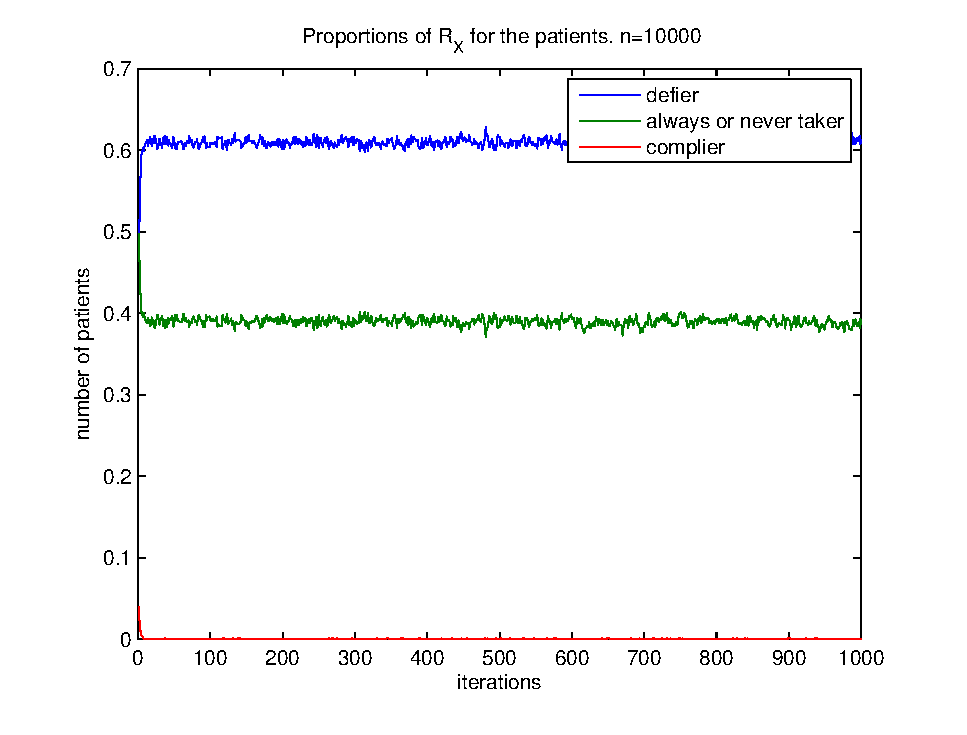
\includegraphics[width=4.5cm,height=4cm,bb=103 240 500
555]{takingtype_case0.38_0.78_n=10000.eps} &
 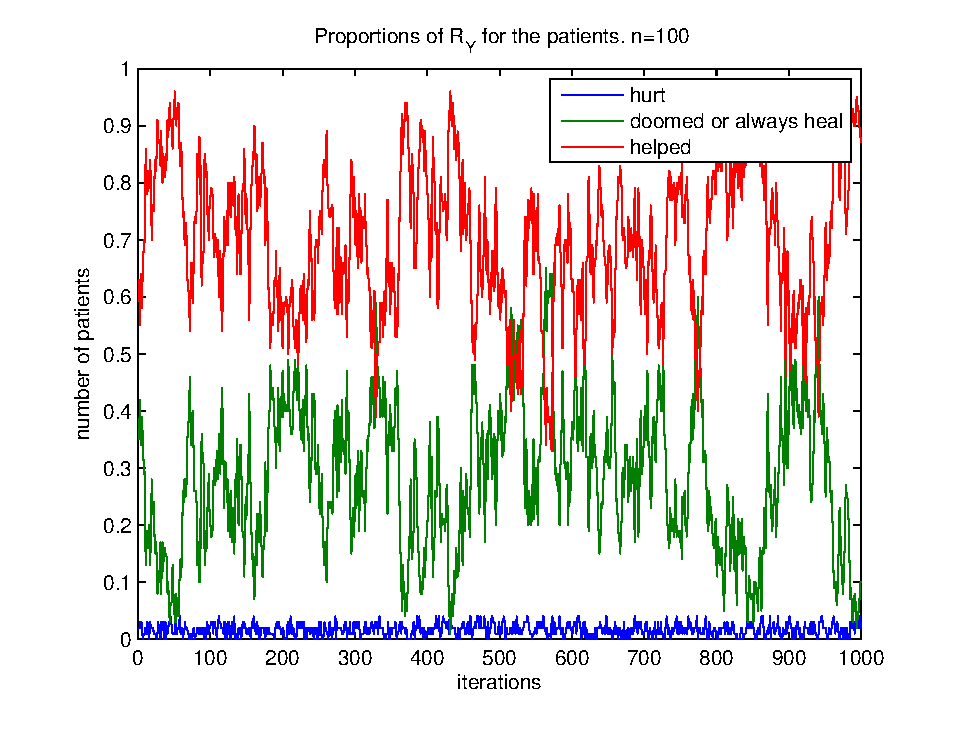
\includegraphics[width=4.5cm,height=4cm,bb=103 240 500 555]
{healingtype_case0.38_0.78_n=100.eps} &
 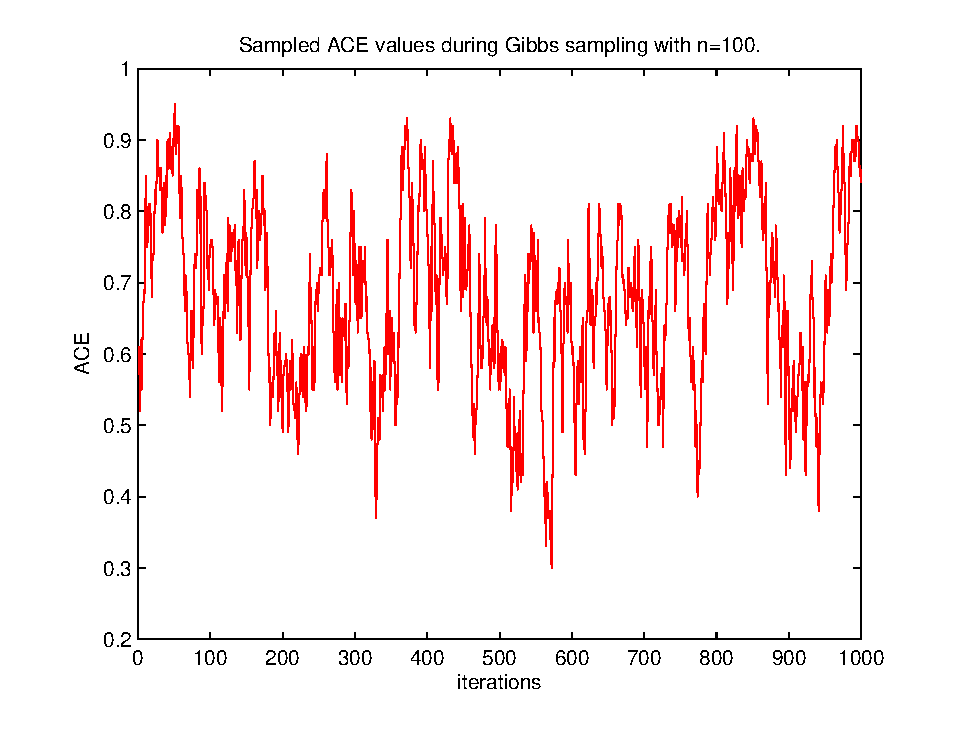
\includegraphics[width=4.5cm,height=4cm,bb=103 240
500 555]{sampledACEs_case0.38_0.78_n=100.eps} \\
(a) & (b) & (c)
\end{tabular}
\caption{Different categories of patients assigned during Gibbs sampling. We
have sampled $n=100$ patients from a distribution that should produce an
unidentifiable ACE in $[0.38, 0.78]$.}
\label{fig:n=100_case0.38_0.78}
\end{figure}

\begin{figure}
\begin{tabular}{ccc}
 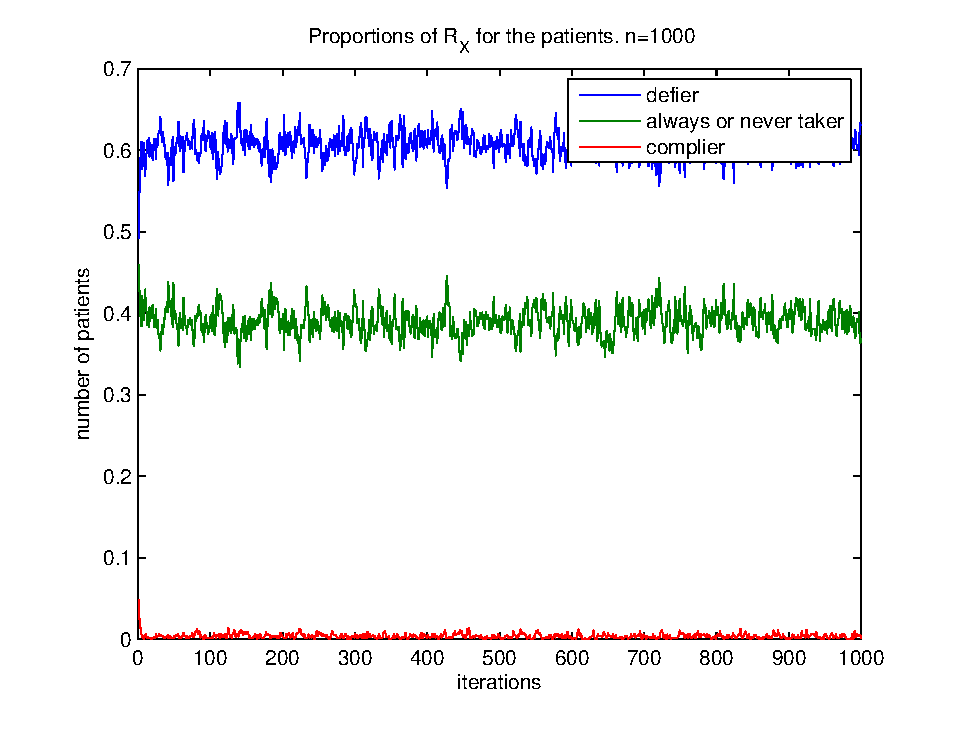
\includegraphics[width=4.5cm,height=4cm,bb=103 240 500
555]{takingtype_case0.38_0.78_n=1000.eps} &
 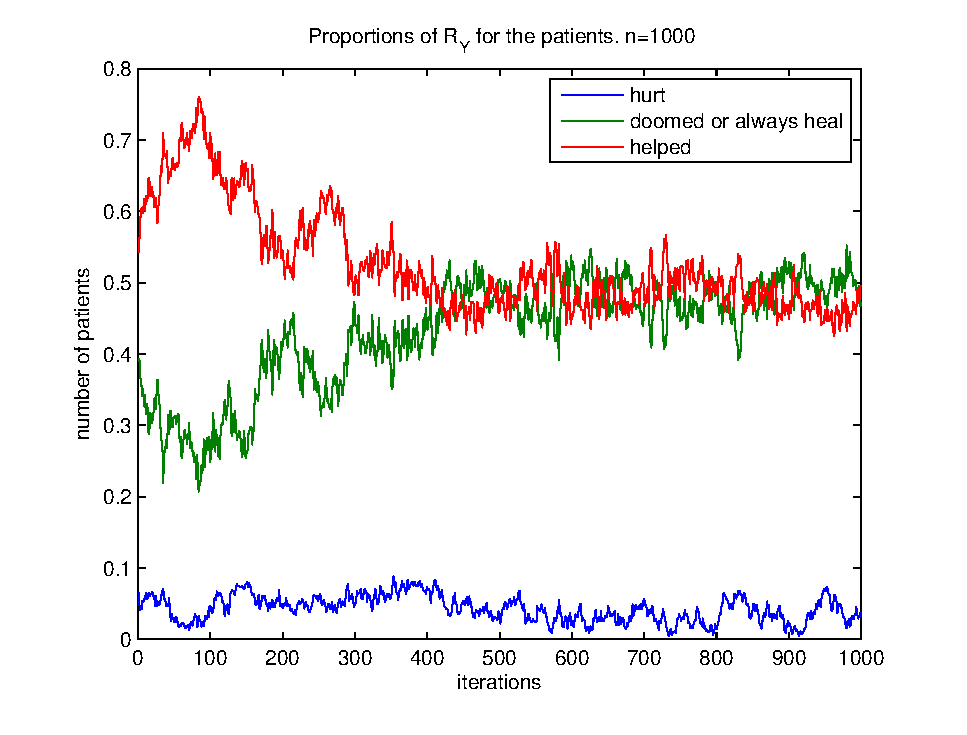
\includegraphics[width=4.5cm,height=4cm,bb=103 240 500 555]
{healingtype_case0.38_0.78_n=1000.eps} &
 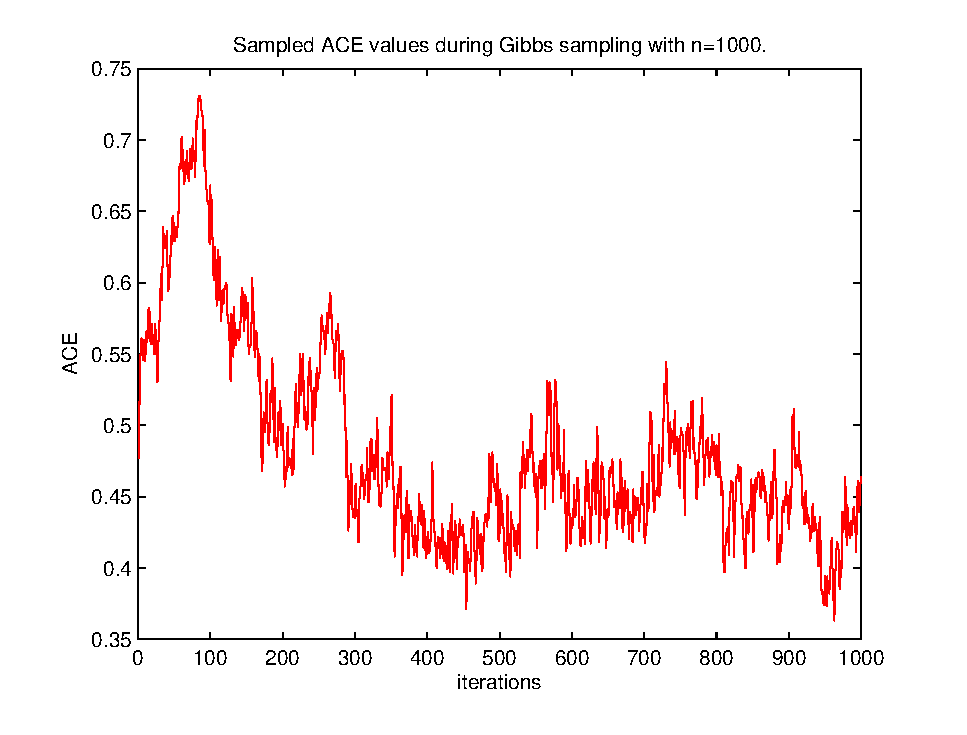
\includegraphics[width=4.5cm,height=4cm,bb=103 240
500 555]{sampledACEs_case0.38_0.78_n=1000.eps} \\
(a) & (b) & (c)
\end{tabular}
\caption{Different categories of patients assigned during Gibbs sampling. We
have sampled $n=1\ 000$ patients from a distribution that should produce an
unidentifiable ACE in $[0.38, 0.78]$.}
\label{fig:n=1000_case0.38_0.78}
\end{figure}

\begin{figure}
\begin{tabular}{ccc}
 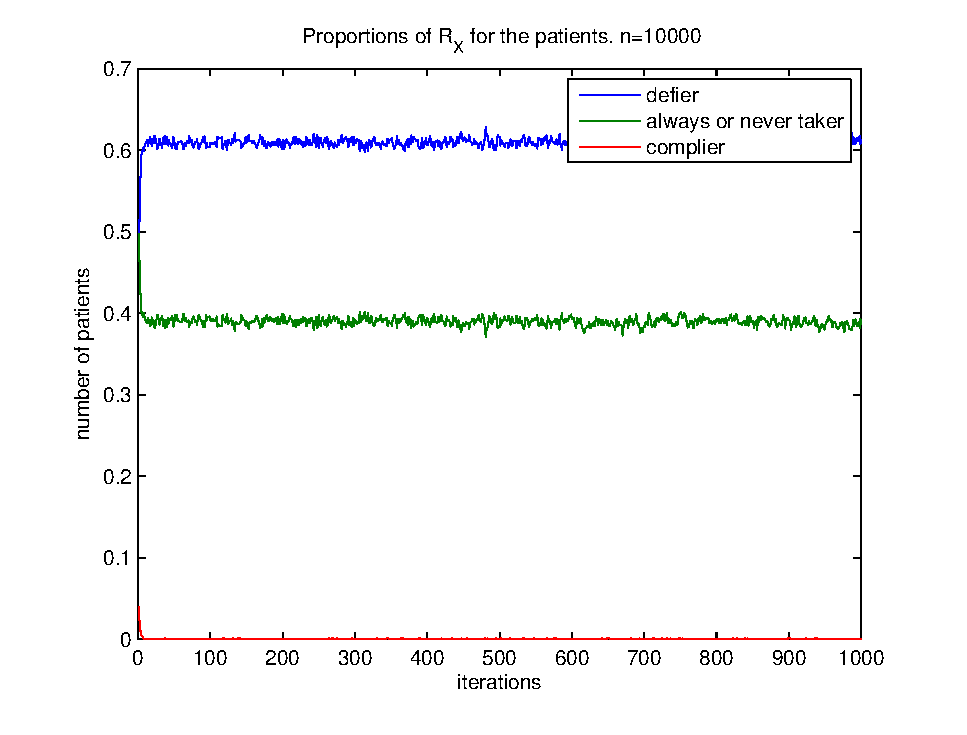
\includegraphics[width=4.5cm,height=4cm,bb=103 240 500
555]{takingtype_case0.38_0.78_n=10000.eps} &
 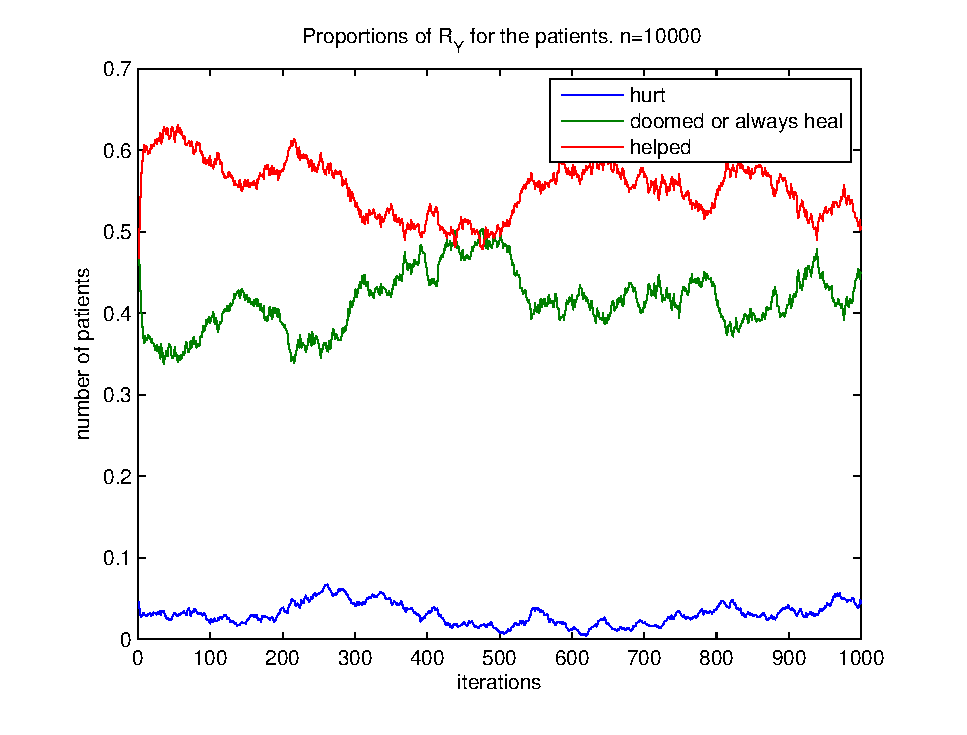
\includegraphics[width=4.5cm,height=4cm,bb=103 240 500 555]
{healingtype_case0.38_0.78_n=10000.eps} &
 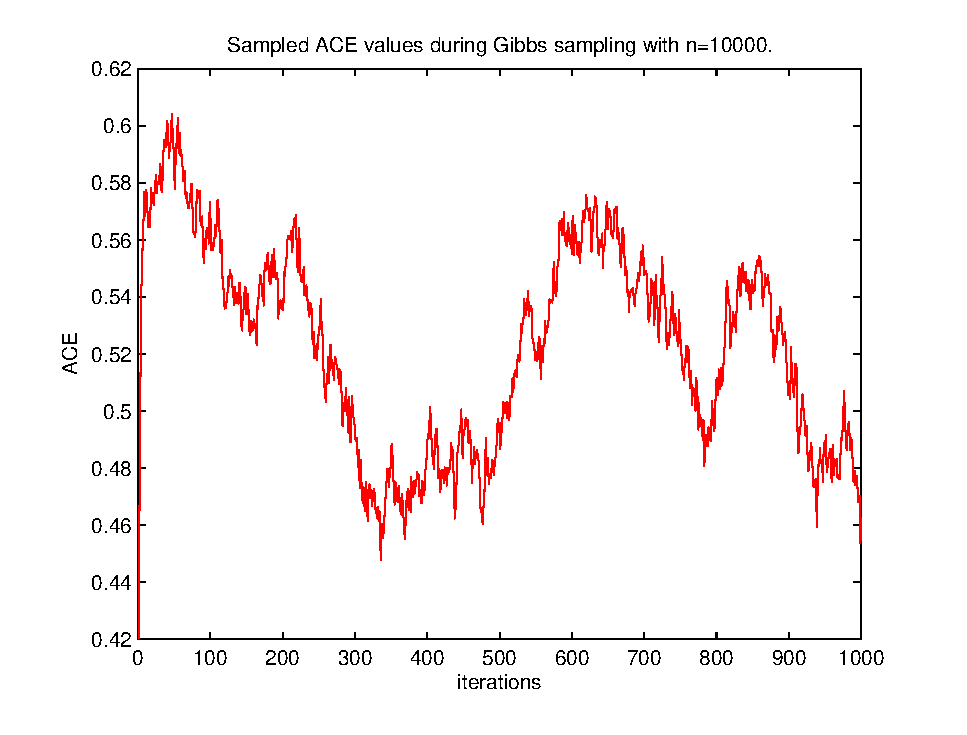
\includegraphics[width=4.5cm,height=4cm,bb=103 240
500 555]{sampledACEs_case0.38_0.78_n=10000.eps} \\
(a) & (b) & (c)
\end{tabular}
\caption{Different categories of patients assigned during Gibbs sampling. We
have sampled $n=10\ 000$ patients from a distribution that should produce an
unidentifiable ACE in $[0.38, 0.78]$ .}
\label{fig:n=10000_case0.38_0.78}
\end{figure}

The graphics presented here use a prior of $\alpha = (1, \ldots, 1)$, but other
priors are also valid. Selecting a good prior is hard because of the complexity
of the relations encapsulated in $U$. The fact that many patients are
``defiers'' $(R_X=2)$ in
figures \ref{fig:n=100_case0.38_0.78},
\ref{fig:n=1000_case0.38_0.78} and \ref{fig:n=10000_case0.38_0.78} has
more to do with their initial reaction to the treatment than their rebelious
personalities. If the drug was hard to obtain, or if
avoiding the assigned treatment required much efforts, we could imagine
selecting a prior to encode this belief.

We should note, too, that $ACE(X\rightarrow Y) \in [0.38, 0.78]$ is still a
strong result. The choice of examples presented in this paper suggests that the
values for $ACE(X\rightarrow Y)$ are always high, but when we sample values of
$Q$ from a Dirichlet distribution with $\alpha_1 = \ldots = \alpha_{16}$, we get
an average of 0 for $ACE(X\rightarrow Y)$.

We can also see that although $ACE(X\rightarrow Y)$ was not identifiable in
figures \ref{fig:n=100_case0.38_0.78},
\ref{fig:n=1000_case0.38_0.78} and \ref{fig:n=10000_case0.38_0.78}, we got in
the first graphs (a) a concentrated posterior distribution for the number of
defiers/compliers. That itself leads to interesting questions about the
treatment being studied.

Finally, we should note that the value $ACE(X\rightarrow Y)$ that we studied in
this paper is used to evaluate how many more people would recover if we applied
the treatment $(\textit{do}(X=1))$ to everyone. Even with a
positive $ACE(X\rightarrow Y)$, it might still be smarter to let people have
their own say, thought such a thing might not always be possible (ex : water
fluoridation). A patient with a strong averse reaction to a treatment might not
care if the treatment is going to have positive (or negligible) effects for
99\% of his neighbors.

These questions fall outside the scope of the current review. We refer again
the reader to \cite{pearl2000cmr} that offers basic methods to evaluate certain
counterfactual statements.

The choice of $ACE(X\rightarrow Y) = p(R_Y=2) - p(R_Y=3)$ as the object of
study is also arguable. We are all familiar with what
``twice as many chances of succeeding'' means, but an increase of $5\%$ in
probabilities has to be put in context. Having $1\%$ more chances of
winning the lottery is enormous, but having $1\%$ more chances of winning a
meaningless one-time coin flip is negligible. The current
definition of the $ACE(X\rightarrow Y)$ is convenient when considering the
effects of a policy change on a population to determine how many more
individuals would be positively affected. But when $X$ involves a significant
cost, $ACE(X\rightarrow Y)$ needs to be put into context. We would readily pay
$\$100$ to have an increase of $+1\%$ in absolute odds for the lottery, going
from $0\%$ to $1\%$.

%\section{Conclusion}

\bibliography{stat561project}

\end{document}
